\fancyhead{}
\fancyfoot{}
\pagestyle{plain}

\lhead{Método}

\chapter{Método}

Este capítulo describe el desarrollo del trabajo de investigación, enfocado en la creación de un prototipo de control para motocicletas mediante tecnologías \textit{\acrshort{rfid-acronym}} y \textit{\acrshort{loraw}}, con el propósito de implementar un sistema de autenticación y localización para prevenir robos. El trabajo constituye una investigación aplicada al desarrollo tecnológico de un sistema de seguridad antirrobo, con un enfoque cuantitativo y un diseño experimental y transversal en el tiempo, abarcando el desarrollo de un prototipo funcional. En las siguientes secciones se detallan los módulos desarrollados, cada uno representando una fase clave en el funcionamiento del sistema (ver Figura \ref{modulo}).

\begin{figure}[H]
    \centering
    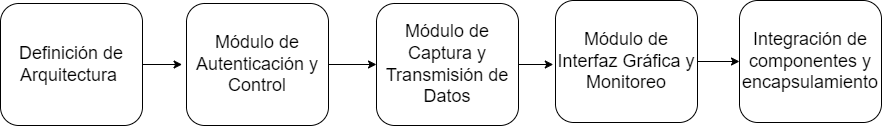
\includegraphics[width=\textwidth]{./capitulo_04/imagen/modulos.drawio.png}
    \caption{Fases principales del sistema.}
    \label{modulo}
\end{figure}

\section{Definición de arquitectura}

En esta primera fase, se definieron los requisitos técnicos orientados a proporcionar seguridad y monitoreo remoto en tiempo real mediante tecnologías \textit{IoT}. El objetivo principal fue desarrollar un sistema que autentique al propietario de la motocicleta a través de un módulo \textit{\acrshort{rfid-acronym}} y, en caso de intento de robo o alejamiento del vehículo sin el \textit{tag} autorizado, interrumpa el encendido y envíe una alerta a un servidor remoto. Para satisfacer estos requisitos, se diseñó una arquitectura que integra comunicación de baja potencia mediante \textit{\acrshort{loraw}} y un dispositivo de geolocalización \textit{\acrshort{gnss-acronym}}, permitiendo el monitoreo y la visualización de datos en una plataforma gráfica accesible.

\subsection{Requisitos clave}

\begin{itemize}
    \item Autenticación del propietario mediante \textit{\acrshort{rfid-acronym}}.
    \item Corte de corriente en el sistema de encendido de la motocicleta cuando el \textit{tag} autorizado se encuentre fuera de rango.
    \item Envío de datos de geolocalización (coordenadas \textit{\acrshort{gnss-acronym}}) y estado de autenticación mediante \textit{\acrshort{loraw}} hacia la red Helium.
    \item Monitoreo remoto de la ubicación y estado de la motocicleta a través de una interfaz gráfica.
\end{itemize}

Con base en estos requisitos, se definieron dos aspectos principales: la estructura interna del prototipo y la arquitectura de comunicación externa hacia el servidor. 

\subsection{Estructura interna del prototipo}

La Figura \ref{fig:diagrama1} ilustra el diseño del hardware y el flujo de control dentro del prototipo.

\begin{figure}[H]
\leavevmode
\begin{minipage}{\textwidth}
\begin{center}
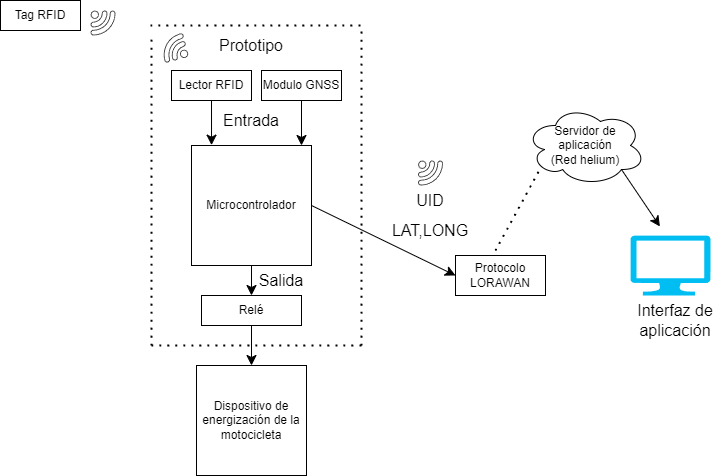
\includegraphics[scale=0.5]{./capitulo_04/imagen/diagrama1.png}
\caption{Estructura del prototipo. \label{fig:diagrama1}}
\end{center}
\end{minipage}
\end{figure}

\begin{itemize}
    \item \textbf{Microcontrolador (Heltec WiFi LoRa 32 V3):} Procesa las entradas de los módulos \textit{\acrshort{rfid-acronym}} y \textit{\acrshort{gnss-acronym}}, y envía datos mediante \textit{\acrshort{loraw}}.
    \item \textbf{Módulo \textit{\acrshort{rfid-acronym}}:} Detecta y autentica el \textit{tag} del usuario. Si el \textit{UID} del \textit{tag} coincide con uno de los usuarios autorizados, se habilita el sistema de arranque.
    \item \textbf{Módulo \textit{\acrshort{gnss-acronym}}:} Proporciona las coordenadas de geolocalización, que se envían junto con el \textit{UID} autenticado para monitoreo remoto.
    \item \textbf{Relé:} Controla el flujo de energía hacia el encendido de la motocicleta. Si el \textit{tag \acrshort{rfid-acronym}} no es reconocido o se retira del rango, el relé corta la energía, evitando que la motocicleta arranque.
\end{itemize}

\subsection{Arquitectura de comunicación externa}

La Figura \ref{fig:diagrama2} muestra cómo los datos capturados por el prototipo se procesan para cumplir con los requisitos de monitoreo remoto en tiempo real.

\begin{figure}[H]
\leavevmode
\begin{minipage}{\textwidth}
\begin{center}
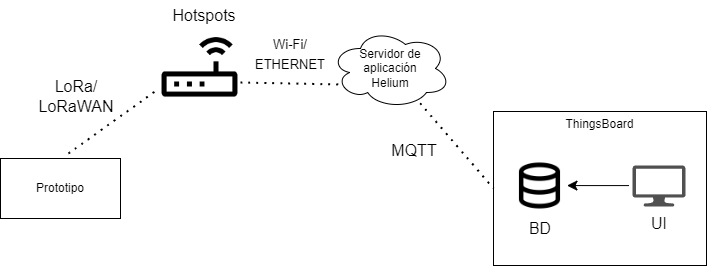
\includegraphics[scale=0.5]{./capitulo_04/imagen/diagrama2.png}
\caption{Arquitectura de comunicación y monitoreo. \label{fig:diagrama2}}
\end{center}
\end{minipage}
\end{figure}

\begin{itemize}
    \item \textbf{Prototipo:} Recopila datos del \textit{\acrshort{rfid-acronym}} y las coordenadas \textit{\acrshort{gnss-acronym}}. El microcontrolador envía esta información utilizando el protocolo \textit{\acrshort{loraw}}.
    \item \textbf{\textit{Hotspots Helium}:} Actúan como puntos de acceso, recibiendo los datos enviados por el prototipo y transmitiéndolos al servidor de aplicación.
    \item \textbf{Servidor Helium:} Procesa los datos recibidos y los envía mediante el protocolo \textit{MQTT} a la plataforma \textit{ThingsBoard}.
    \item \textbf{\textit{ThingsBoard (UI):}} Plataforma que permite la visualización gráfica de los datos en tiempo real. Los usuarios pueden monitorear la ubicación de la motocicleta, su estado de autenticación, y recibir alertas en caso de eventos inusuales, como intentos de robo.
\end{itemize}


\section{Módulo de autenticación y control}

En esta fase, se desarrollaron las funciones principales para garantizar la autenticación del usuario antes de permitir el arranque de la motocicleta. El sistema está diseñado para validar la presencia de un \textit{tag \acrshort{rfid-acronym}} autorizado; solo cuando se detecta un \textit{tag} registrado se permite el arranque del motor de la motocicleta. Si el \textit{tag} no es detectado o es removido en algún momento, el sistema corta el suministro de corriente al motor, bloqueando su funcionamiento. Este mecanismo proporciona una primera capa de seguridad para prevenir el uso no autorizado de la motocicleta.

\subsection{Requisitos del sistema}

Para implementar esta funcionalidad, se definieron los siguientes requisitos:

\begin{itemize}
    \item \textbf{Comparación de UID:} El sistema debe comparar el UID del \textit{tag} detectado con una lista de UID autorizados.
    \item \textbf{Verificación en rango:} Una vez autorizado el \textit{tag}, el sistema realiza una lectura constante para verificar que el \textit{tag} permanezca en rango.
\end{itemize}

Considerando estos requisitos, se diseñó el diagrama de flujo que representa el funcionamiento del sistema de autenticación y control (Figura \ref{fig:rfid1}).

\begin{figure}[H]
    \centering
    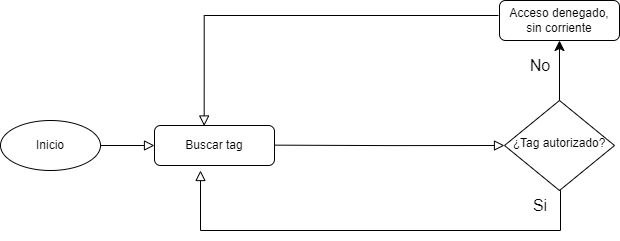
\includegraphics[scale=0.5]{./capitulo_04/imagen/diagramadeflujoRFID-Page-1.drawio.png}
    \caption{Diagrama de flujo de autenticación y control.}
    \label{fig:rfid1}
\end{figure}

\subsection{Conexión del módulo \textit{RFID}}

Para la comunicación entre el módulo \textit{RFID RC522} y la placa de desarrollo \textit{WiFi LoRa 32 V3} se empleó el protocolo SPI. Los pines de conexión utilizados fueron: 
\begin{itemize}
    \item \textbf{CS:} Pin 34.
    \item \textbf{MOSI:} Pin 35.
    \item \textbf{CLK:} Pin 36.
    \item \textbf{MISO:} Pin 26.
    \item \textbf{RESET:} Pin 33.
    \item \textbf{VCC y GND:} Pines de alimentación.
\end{itemize}

En la Figura \ref{fig:conexionrfid} se muestra el diagrama de conexiones utilizadas para esta configuración.

\begin{figure}[H]
\leavevmode
\begin{minipage}{\textwidth}
\begin{center}
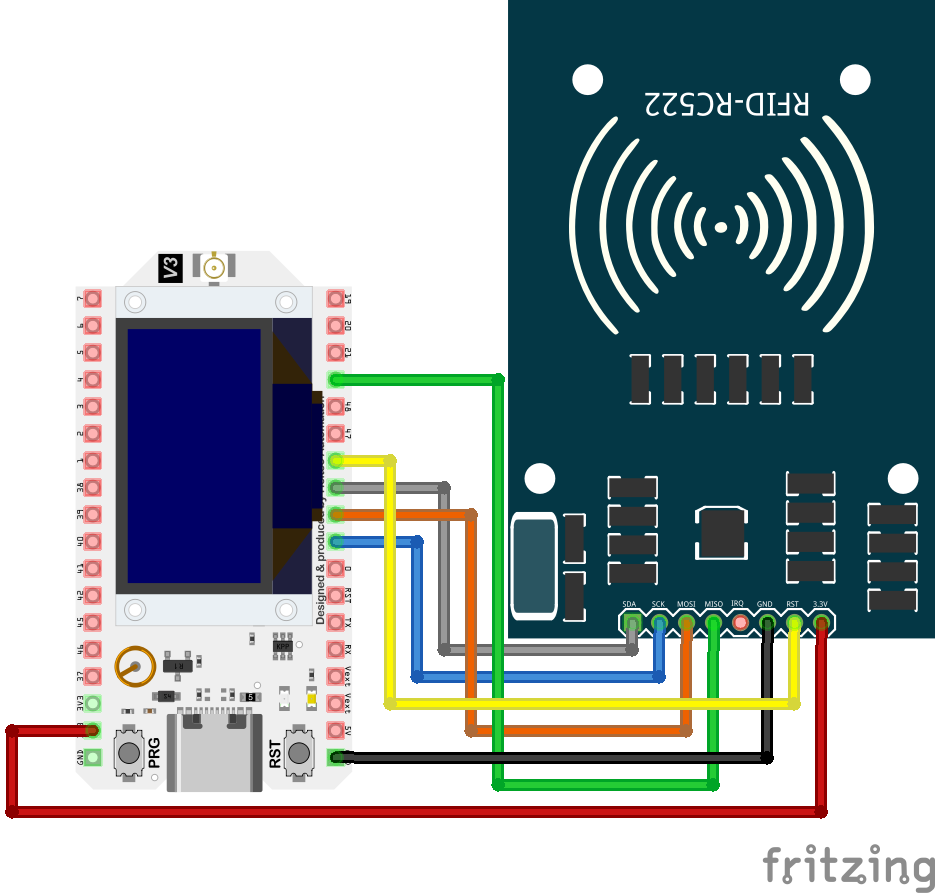
\includegraphics[scale=0.8]{./capitulo_04/imagen/diagramaRFID.png}
\caption{Diagrama de conexiones entre WiFi LoRa 32 V3 y RFID RC522. \label{fig:conexionrfid}}
\end{center}
\end{minipage}
\end{figure}

\subsection{Primera versión del código: implementación básica en el bucle principal}

La primera versión del código implementa un sistema de autenticación y monitoreo continuo de un \textit{tag \acrshort{rfid-acronym}}, permitiendo el acceso únicamente cuando se detecta la presencia de un \textit{tag} autorizado. En este caso, se definieron dos UIDs correspondientes a \textit{Usuario1} y \textit{Usuario2}. Al leer el UID del \textit{tag}, el sistema lo compara con estos valores autorizados para conceder o denegar el acceso.

\subsubsection{Autenticación del \textit{tag}}
\begin{itemize}
    \item Si \texttt{tagAutenticada} es \texttt{falso}, el sistema permanece en espera, buscando la presencia de un \textit{tag \acrshort{rfid-acronym}}.
    \item Cuando se detecta un \textit{tag}, se lee su UID y se utiliza la función \texttt{comparaUID()} para verificar si coincide con uno de los usuarios autorizados. Si coincide, se muestra un mensaje de bienvenida y \texttt{tagAutenticada} se establece en \texttt{verdadero}.
    \item Si el UID no es reconocido, se muestra un mensaje indicando que el \textit{tag} no es válido.
\end{itemize}

\subsubsection{Verificación de presencia del \textit{tag}}
\begin{itemize}
    \item Si \texttt{tagAutenticada} es \texttt{verdadero}, el sistema verifica constantemente si el \textit{tag} autorizado permanece en rango.
    \item Si el tiempo desde la última detección del \textit{tag} excede un límite definido (\texttt{tiempoCorte}), el sistema corta el suministro de corriente al motor.
    \item Si el \textit{tag} sigue en rango, se actualiza el tiempo de última lectura y el motor continúa en funcionamiento.
\end{itemize}

\subsection{Segunda versión del código: integración de FreeRTOS y modularización}

En esta versión, se incorporó \gls{rtos} para gestionar de manera concurrente la autenticación del \textit{tag \acrshort{rfid-acronym}} y la verificación de su presencia. Además, el código se modularizó en archivos específicos para facilitar su mantenimiento y escalabilidad:

\begin{itemize}
    \item \textbf{Archivo \texttt{rfidfunciones.h}:} Declaraciones de variables y funciones relacionadas con el módulo \textit{\acrshort{rfid-acronym}}.
    \item \textbf{Archivo \texttt{rfidfunciones.cpp}:} Implementación de funciones y tareas de FreeRTOS para autenticación y monitoreo.
    \item \textbf{Archivo principal \texttt{RFIDFreeRTOS.ino}:} Inicialización de tareas de FreeRTOS y configuración de parámetros principales.
\end{itemize}

\subsubsection{Tareas implementadas con FreeRTOS}

\paragraph{Tarea 1: \texttt{tareaDeteccionTag}}
\begin{itemize}
    \item Busca la presencia de un \textit{tag \acrshort{rfid-acronym}}. Si se detecta, verifica su autenticidad mediante la función \texttt{autenticarTag()}.
    \item Monitorea la permanencia del \textit{tag} en rango. Si el \textit{tag} es detectado nuevamente, actualiza el tiempo de última lectura.
    \item Notifica a la tarea de verificación del tiempo mediante un semáforo (\texttt{tagDetectadaSemaphore}).
\end{itemize}

\paragraph{Tarea 2: \texttt{tareaVerificarTiempo}}
\begin{itemize}
    \item Espera la señal del semáforo para ejecutar la función \texttt{verificarTiempo()}, que comprueba si el tiempo transcurrido desde la última detección supera el límite definido (\texttt{tiempoCorte}).
    \item Si el tiempo excede el límite, se corta el suministro de corriente y se establece \texttt{tagAutenticada} en \texttt{falso}.
\end{itemize}

Esta versión proporciona una estructura modular, mejorando la eficiencia y permitiendo un control más preciso del sistema. El uso de \textit{FreeRTOS} optimiza la gestión de tareas críticas, asegurando la sincronización y escalabilidad del sistema.


\section{Módulo de captura y transmisión de datos}

Para llevar a cabo la captura y transmisión de datos en tiempo real, se desarrollaron códigos específicos que permiten la adquisición de coordenadas de ubicación mediante el módulo \textit{\acrshort{gnss-acronym}} y su transmisión eficiente a través de \textit{\acrshort{loraw}}, integrando ambos subsistemas en el funcionamiento general del prototipo.

Este proceso se dividió en tres fases:

\begin{itemize}
    \item Implementación básica para obtención de datos de las coordenadas en tiempo real.
    \item Implementación y configuración del módulo \textit{\acrshort{loraw}} para la transmisión de datos.
    \item Integración de la comunicación entre los módulos \textit{\acrshort{gnss-acronym}} y \textit{\acrshort{loraw}}.
\end{itemize}

Para la comunicación entre el módulo \textit{\acrshort{gnss-acronym}} y la placa de desarrollo \textit{WiFi LoRa 32 V3}, se empleó el protocolo \textit{UART}. Los pines de conexión utilizados fueron el pin 45 (RX), pin 46 (TX), y los pines de alimentación \textit{VCC} y \textit{GND}. En la Figura \ref{fig:conexionGNSS}, se muestra el diagrama de conexiones utilizado.

\begin{figure}[H]
    \leavevmode
    \begin{minipage}{\textwidth}
    \begin{center}
    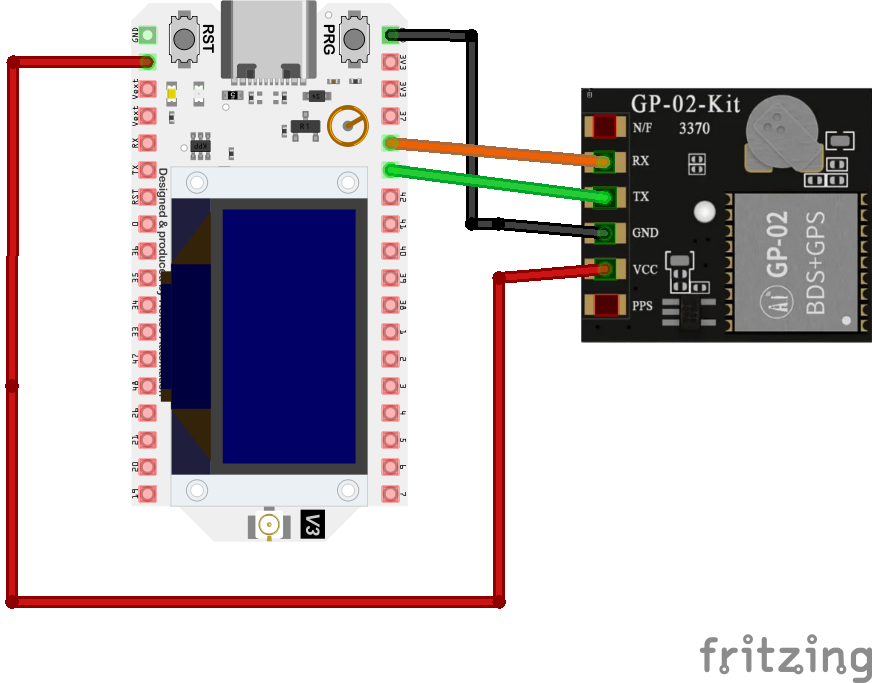
\includegraphics[scale=0.8]{./capitulo_04/imagen/diagramaGNSS.png}
    \caption{Diagrama de conexiones entre \textit{WiFi LoRa 32 V3} y \textit{\acrshort{gnss-acronym}}. \label{fig:conexionGNSS}}
    \end{center}
    \end{minipage}
\end{figure}

\subsection{Implementación básica para obtención de datos de las coordenadas en tiempo real}

Una vez conectado el módulo \textit{\acrshort{gnss-acronym}} a la placa de desarrollo, se implementó un código para obtener y mostrar en tiempo real los datos de ubicación (latitud y longitud), junto con la fecha y hora actual. Este código se basa en la librería \textit{TinyGPSPlus}, que permite interpretar los datos en formato \textit{NMEA} recibidos desde el GPS. A continuación, se describe la implementación:

\subsubsection{Función \texttt{setup()}}
Durante la fase de inicialización, la función \texttt{setup()} se encarga de:
\begin{itemize}
    \item Configurar el monitor serial (\texttt{Serial}) a 115200 baudios para facilitar la visualización de los datos en una terminal serial.
    \item Configurar \texttt{Serial1}, el puerto serial dedicado a la comunicación con el GPS, con los pines y velocidad previamente definidos.
\end{itemize}

\subsubsection{Proceso de captura de datos en la función \texttt{loop()}}

En la función \texttt{loop()}, el sistema verifica continuamente si hay datos disponibles en el puerto \texttt{Serial1}, donde el módulo \textit{GPS} envía sus mensajes de datos. El flujo de trabajo en esta función es el siguiente:

\paragraph{Recepción y decodificación de datos:}
\begin{itemize}
    \item Cuando \texttt{Serial1} tiene datos disponibles, estos se procesan utilizando la función \texttt{gps.encode()}. Esta función decodifica los mensajes de datos en formato \textit{NMEA} provenientes del \textit{GPS} y almacena la información en la instancia \texttt{gps} de la clase \textit{TinyGPSPlus}.
\end{itemize}

\paragraph{Verificación de la validez de los datos:}
\begin{itemize}
    \item Si \texttt{gps.encode()} detecta un mensaje completo de datos \textit{GPS} válido, se llama a la función \texttt{displayInfo()}, que muestra los datos procesados (ubicación, fecha y hora) en el monitor serial.
    \item Si no se reciben suficientes caracteres de \textit{GPS} dentro de los primeros 5 segundos (menos de 10 caracteres), se muestra un mensaje de error en el monitor serial indicando que no se detecta el \textit{GPS}. Esto podría deberse a un problema de cableado, en cuyo caso el sistema se detiene para evitar lecturas incorrectas.
\end{itemize}

\subsubsection{Función \texttt{displayInfo()}}

La función \texttt{displayInfo()} se encarga de presentar los datos de ubicación, fecha y hora en el monitor serial.

\paragraph{Visualización de la ubicación (latitud y longitud):}
\begin{itemize}
    \item Si los datos de ubicación son válidos (\texttt{gps.location.isValid()}), se muestran la latitud y longitud con una precisión de hasta seis decimales. Esta precisión permite obtener coordenadas exactas del dispositivo en el mapa.
    \item Si los datos no son válidos, se muestra el mensaje “\texttt{INVALIDO}” en lugar de las coordenadas.
\end{itemize}

\paragraph{Visualización de la fecha:}
\begin{itemize}
    \item Si el \textit{GPS} proporciona una fecha válida (\texttt{gps.date.isValid()}), esta se presenta en formato \texttt{MM/DD/AAAA}.
    \item Si la fecha no es válida o no se ha recibido, se muestra “\texttt{INVALIDO}” en su lugar.
\end{itemize}

\paragraph{Visualización de la hora:}
\begin{itemize}
    \item La hora se muestra en formato \texttt{HH:MM:SS.CC} (horas, minutos, segundos y centésimas de segundo) si los datos son válidos (\texttt{gps.time.isValid()}).
    \item Si la hora no es válida, se muestra “\texttt{INVALIDO}”.
\end{itemize}



\subsection{Implementación y configuración del módulo \acrshort{loraw} para la transmisión de datos}

En esta fase, se llevó a cabo la configuración del sistema de transmisión de datos mediante la consola \textit{Helium (Legacy)} \cite{Helium_Console}, junto con la placa de desarrollo Heltec WiFi LoRa 32 V3. A continuación, se detallan los pasos y configuraciones necesarios para establecer la comunicación entre el dispositivo y la red \textit{Helium}, así como los procesos requeridos para su correcto funcionamiento.

\subsubsection{Uso de la consola \textit{Helium}}
La consola \textit{Helium} se empleó para configurar los parámetros de los nodos, verificar el estado de la red y monitorear las transmisiones de datos. A través de esta plataforma, se prepararon los entornos necesarios para visualizar la conectividad entre los dispositivos y la consola, incluyendo el registro de los dispositivos y la verificación de su comunicación con los \textit{gateways}.

El proceso comenzó con el acceso a una organización en la que se habían otorgado permisos de usuario. Tras recibir estos permisos, se procedió a crear una cuenta en la plataforma \textit{Helium}. Completado el registro y acceso a la cuenta, fue posible crear un nodo en la red \textit{Helium}, configurado específicamente para recibir los datos transmitidos por el dispositivo. La Figura \ref{fig:helium} ilustra el entorno de configuración en la consola \textit{Helium}, donde se han resaltado con recuadros negros los elementos clave, incluyendo las credenciales principales necesarias para establecer la conexión.

\begin{figure}[H]
\leavevmode
\begin{minipage}{\textwidth}
\begin{center}
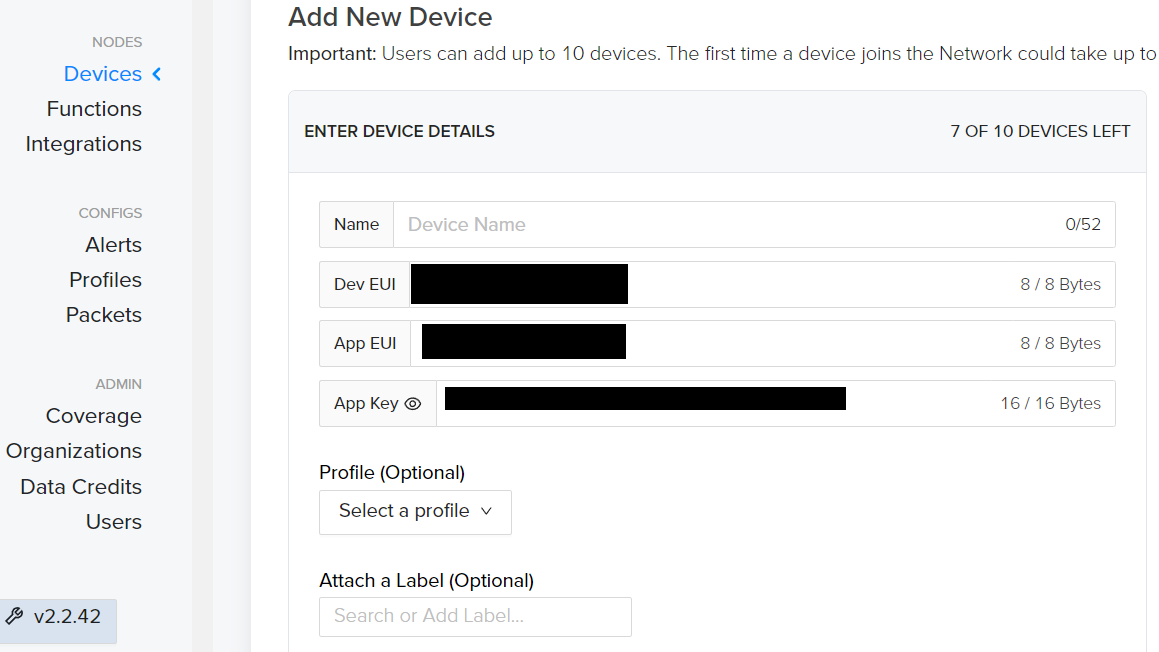
\includegraphics[width=\textwidth]{./capitulo_04/imagen/helium.png}
\caption{Entorno para crear dispositivo y configuración de las credenciales necesarias para el nodo. \label{fig:helium}}
\end{center}
\end{minipage}
\end{figure}

\subsubsection{Configuración del dispositivo Heltec WiFi LoRa 32 V3}

Luego de crear el nodo y obtener las credenciales necesarias, el siguiente paso fue la configuración de la placa de desarrollo Heltec WiFi LoRa 32 V3. Para la implementación inicial, se utilizó la documentación oficial de \textit{Heltec Automation} \cite{heltec}, que proporciona instrucciones detalladas paso a paso sobre la configuración del módulo \textit{\acrshort{loraw}}, así como las librerías requeridas para su funcionamiento.

Una vez completada esta configuración, se consultó la guía oficial de \textit{Helium} \cite{heliumDocs1}, para su integración en el entorno Arduino IDE, adaptándola a las especificaciones particulares de la placa. Esta guía proporcionó los pasos necesarios para registrar las credenciales generadas, permitiendo que el dispositivo enviara datos en \textit{uplink} a la red \textit{Helium}. En la Figura \ref{fig:dispositivo}, se muestran los ajustes de los parámetros necesarios para la comunicación con el servidor \textit{\acrshort{loraw}}.

\begin{figure}[H]
\leavevmode
\begin{minipage}{\textwidth}
\begin{center}
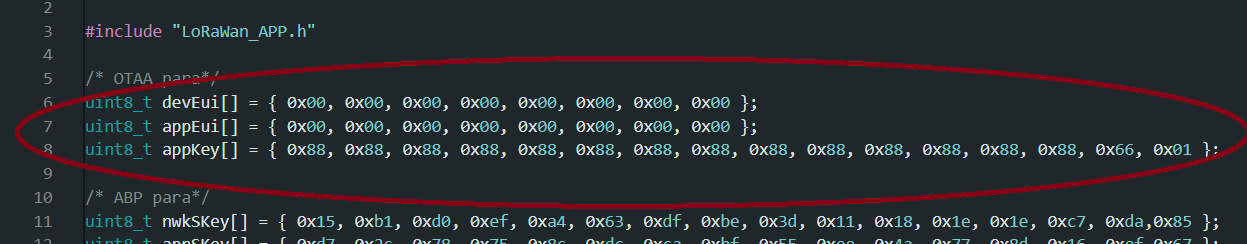
\includegraphics[width=\textwidth]{./capitulo_04/imagen/otta.png}
\caption{Ajuste de los parámetros necesarios en el dispositivo para la comunicación con el servidor \textit{\acrshort{loraw}}. \label{fig:dispositivo}}
\end{center}
\end{minipage}
\end{figure}


\subsection{Implementación de la comunicación entre los módulos\textit{\acrshort{gnss-acronym}} y \textit{\acrshort{loraw}}}

Una vez configurados y validados de manera independiente tanto el módulo \textit{\acrshort{gnss-acronym}} como el sistema de comunicación \textit{\acrshort{loraw}}, se procedió con la integración de ambos componentes. El objetivo de esta fase fue garantizar que las coordenadas obtenidas por el módulo \textit{\acrshort{gnss-acronym}} se transmitieran de manera eficiente a través de la red \textit{\acrshort{loraw}}. Para ello, se realizaron los ajustes necesarios en el código, asegurando que la captura de los datos de ubicación y su envío a través de \textit{\acrshort{loraw}} ocurrieran de manera sincronizada y sin pérdida de información.

En esta sección, se describen en detalle los procesos y el funcionamiento del código ajustado para integrar los sistemas de geolocalización y transmisión de datos.

Como primer paso, se diseñó un diagrama de flujo para representar el funcionamiento del sistema integrado, el cual se puede observar en la Figura \ref{fig:flujo}.

\begin{figure}[H]
\leavevmode
\begin{minipage}{\textwidth}
\begin{center}
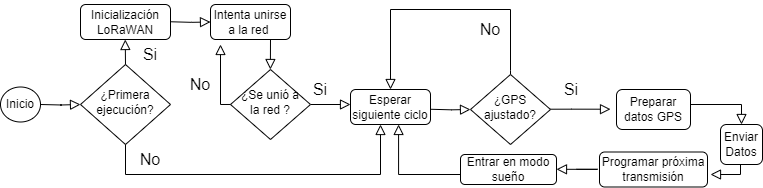
\includegraphics[width=\textwidth]{./capitulo_04/imagen/diagramadeflujognss.png}
\caption{Diagrama de flujo de transmisión de datos por \textit{\acrshort{loraw}}. \label{fig:flujo}}
\end{center}
\end{minipage}
\end{figure}

Una vez diseñado el diagrama de flujo, se procedió a desarrollar una nueva versión del código, reutilizando los fragmentos de código de las fases anteriores e incorporando los ajustes necesarios. A continuación, se describe la implementación de este código.

El programa inicia con la inclusión de las librerías esenciales: \texttt{\acrshort{loraw}APP.h}, para gestionar la comunicación mediante \textit{\acrshort{loraw}}, y \texttt{TinyGPSPlus.h}, para manipular los datos obtenidos del módulo \textit{\acrshort{gnss-acronym}}. Luego, se configuran los pines de acuerdo con las definiciones establecidas en la primera fase del proyecto.

A continuación, se definen los parámetros de conexión de \textit{\acrshort{loraw}}. La conexión puede configurarse de dos maneras: mediante \textit{\acrshort{otaa-acronym}} (\textit{\gls{otaa-glossary}}) o \textit{ABP} (\textit{Activation By Personalization}). Para ello, se especifican las claves necesarias para cada método (\texttt{devEui}, \texttt{appEui}, \texttt{\acrshort{appkey-acronym}} para \textit{\acrshort{otaa-acronym}}, y \texttt{\acrshort{nwkskey-acronym}}, \texttt{\acrshort{appskey-acronym}}, \texttt{devAddr} para \textit{ABP}). También se definen los canales de comunicación y la región de operación.

Posteriormente, se establece un ciclo de transmisión de datos cada 60 segundos (\texttt{appTxDutyCycle} a 60000) y se especifican otros parámetros, como el uso de \textit{ADR} (\textit{Adaptive Data Rate}) y la configuración de los mensajes como confirmados o no confirmados, según los requisitos del sistema.

La función \texttt{prepareTxFrame} se encarga de preparar los datos \textit{GPS} para su envío. Primero, el programa espera hasta obtener una ubicación válida (\texttt{gps.location.isValid()}). Una vez que la señal es válida, la función extrae la latitud y longitud y las almacena en un \textit{buffer} de datos (\texttt{appData}) en el formato adecuado para su transmisión mediante \textit{\acrshort{loraw}}.

Al comenzar el ciclo \texttt{setup}, el programa inicializa la comunicación serie y \textit{\acrshort{loraw}}. Adicionalmente, se utiliza una variable (\texttt{firstrun}) para verificar si es la primera vez que el dispositivo se configura en el \textit{MCU}, mostrando un mensaje en pantalla para confirmar la inicialización.

En el ciclo \texttt{loop}, la lógica del programa sigue una estructura de máquina de estados, que permite gestionar cada fase de la operación \textit{\acrshort{loraw}}. Los estados principales son:

\begin{itemize}
    \item \textbf{DEVICE STATE INIT}: Inicializa el módulo \textit{\acrshort{loraw}} y realiza las configuraciones básicas.
    \item \textbf{DEVICE STATE JOIN}: Intenta unirse a la red \textit{\acrshort{loraw}}, mostrando mensajes de estado.
    \item \textbf{DEVICE STATE SEND}: Llama a \texttt{prepareTxFrame} para obtener y empaquetar los datos de \textit{GPS}, y luego envía la información.
    \item \textbf{DEVICE STATE CYCLE}: Calcula el tiempo hasta la próxima transmisión, usando \texttt{appTxDutyCycle} como base.
    \item \textbf{DEVICE STATE SLEEP}: Pone al dispositivo en modo de bajo consumo para conservar energía hasta la siguiente transmisión.
\end{itemize}

Finalmente, la función \texttt{displayInfo} muestra en el monitor serie la información de ubicación, fecha y hora del \textit{GPS}. En caso de que los datos no estén disponibles, se muestra un mensaje de \textit{INVALIDO}.

\section{Módulo de interfaz gráfica y monitoreo}

El módulo de interfaz gráfica y monitoreo constituye un componente esencial del sistema, proporcionando una plataforma interactiva \textit{IoT} para visualizar en tiempo real la ubicación de la motocicleta y otros parámetros relevantes. Para esta implementación, se utilizó \textit{ThingsBoard Community Edition}, que se conectó a la consola \textit{Helium}, permitiendo la recepción y visualización de los datos transmitidos desde la red. La estructura del módulo incluye un servidor local que procesa y organiza la información en una interfaz gráfica accesible para el usuario final.

La implementación de este módulo se dividió en dos fases principales. La primera fase consistió en la configuración de \textit{ThingsBoard} como receptor de datos, habilitando el procesamiento y la visualización de la información recibida. La segunda fase abordó la integración de la consola \textit{Helium} con \textit{ThingsBoard} mediante el protocolo \textit{MQTT}, configurando un flujo de datos en tiempo real entre el dispositivo y el servidor local.

En las siguientes secciones, se detallan cada una de estas fases:



\subsection{Configuración de \textit{ThingsBoard}}

En esta fase, se llevó a cabo la instalación y configuración de \textit{ThingsBoard} de manera local, siguiendo las instrucciones de la documentación oficial para asegurar una implementación inicial estable \cite{ThingsBoard_docs}. Una vez completada esta instalación, se realizaron configuraciones personalizadas con el objetivo de adaptar la plataforma a los requisitos específicos del sistema de monitoreo.

Los pasos realizados en esta etapa incluyeron:

\paragraph{Creación de dispositivos y configuración de conectividad\\}

En \textit{ThingsBoard}, se añadieron los dispositivos que transmitirían datos al sistema. En este caso, se creó un dispositivo llamado \textit{Poli\_Moto} (ver Figura \ref{fig:tbdisp}) y se le asignó un perfil \textit{MQTT}. Esta configuración permite que el dispositivo envíe datos de telemetría a través de la consola \textit{Helium} hacia \textit{ThingsBoard}.

Se definió un perfil de transporte \textit{MQTT} con los temas de telemetría y atributos configurados para recibir datos en formato \textit{JSON} (ver Figura \ref{fig:tbperfil}). Esto asegura que los datos de ubicación y estado se transmitan de manera continua y en tiempo real.


\begin{figure}[H]
\leavevmode
\begin{minipage}{\textwidth}
\begin{center}
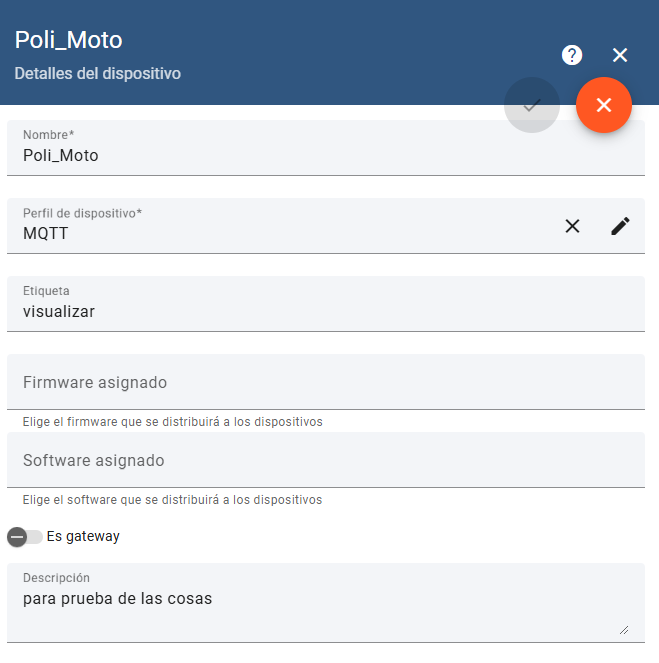
\includegraphics[scale=0.53]{./capitulo_04/imagen/tb/dispositivo.png}
\caption{Detalles del dispositivo ThingsBoard. \label{fig:tbdisp}}
\end{center}
\end{minipage}
\end{figure}

\begin{figure}[H]
\leavevmode
\begin{minipage}{\textwidth}
\begin{center}
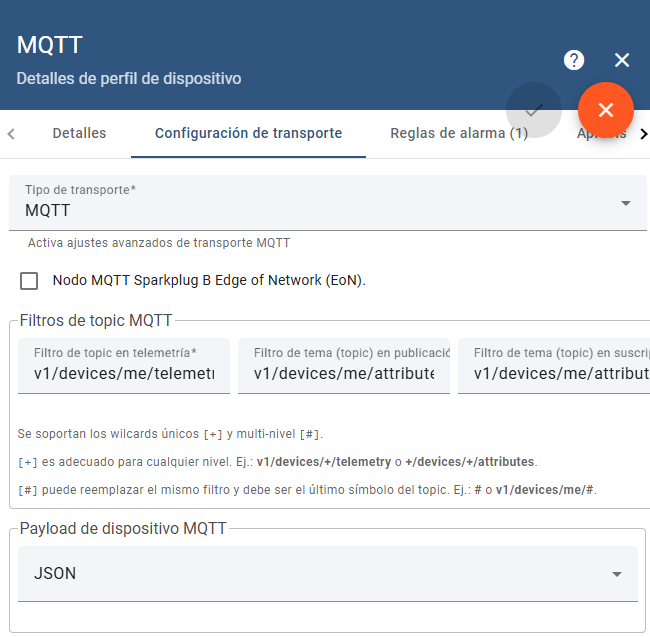
\includegraphics[scale=0.58]{./capitulo_04/imagen/tb/perfil_transport.png}
\caption{Perfil de dispositivo ThingsBoard. \label{fig:tbperfil}}
\end{center}
\end{minipage}
\end{figure}

\paragraph{Gestión de Usuarios y Roles de Acceso\\}

Se crearon diferentes usuarios y clientes para facilitar el acceso y administración de los datos en el sistema. En la configuración de clientes, se creó un cliente de prueba llamado \textit{Cliente\_Prueba}, al cual se le asignaron dispositivos específicos y se configuraron sus permisos de acceso (ver Figuras~\ref{fig:tbclient} y~\ref{fig:tbclient_disp}). 

Se configuraron usuarios con permisos exclusivos para acceder a dispositivos asignados, permitiendo una gestión controlada y personalizada de la información disponible.

\begin{figure}[H]
\leavevmode
\begin{minipage}{\textwidth}
\begin{center}
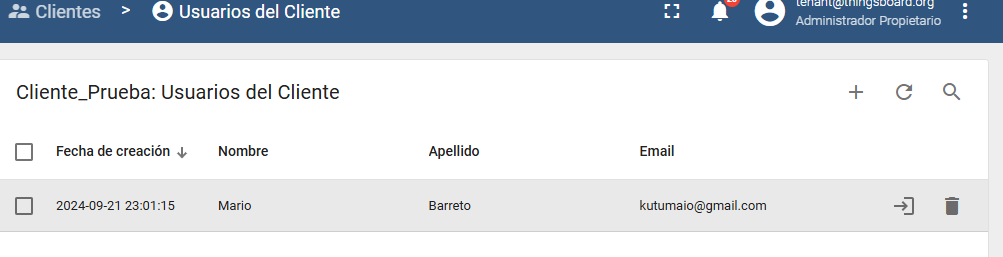
\includegraphics[width=\textwidth]{./capitulo_04/imagen/tb/us_cleint.png}
\caption{Cliente con usuario creado en ThingsBoard. \label{fig:tbclient}}
\end{center}
\end{minipage}
\end{figure}

\begin{figure}[H]
\leavevmode
\begin{minipage}{\textwidth}
\begin{center}
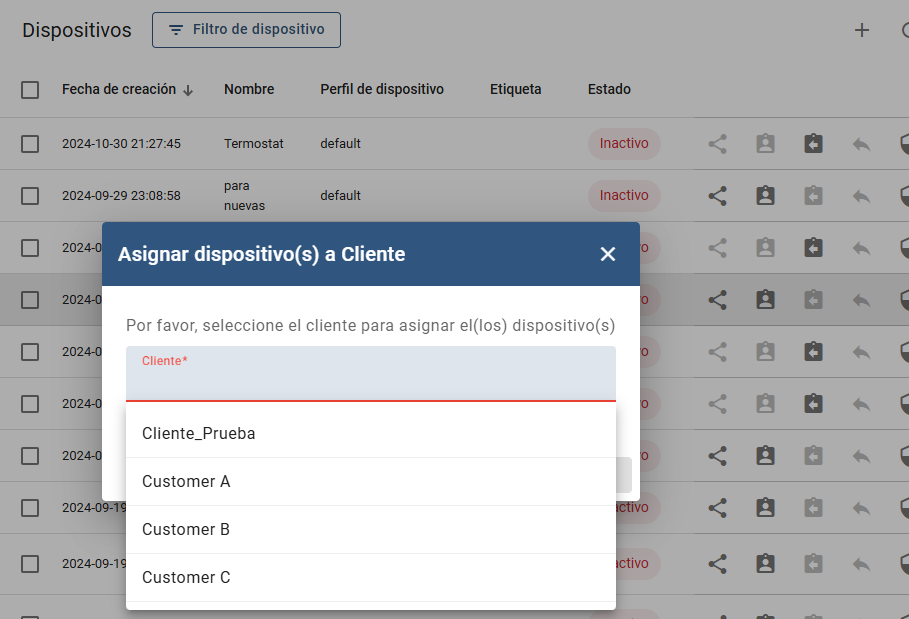
\includegraphics[scale=0.58]{./capitulo_04/imagen/tb/dispos_client.png}
\caption{Asignación de dispositivos a clientes en ThingsBoard. \label{fig:tbclient_disp}}
\end{center}
\end{minipage}
\end{figure}

\paragraph{Diseño del Tablero Interactivo\\}

Se diseñó un tablero personalizado titulado \textit{Mapa\_Mot}, donde se agruparon los datos de los dispositivos en widgets específicos para su monitoreo en tiempo real. Este tablero permite centralizar y visualizar la información de ubicación y otros datos relevantes de los dispositivos conectados.

Se exploraron los \textit{widgets} disponibles en ThingsBoard para elegir aquellos que mejor se adaptaran a las necesidades del sistema (ver Figura \ref{fig:tbpanelelec}). Se seleccionaron los \textit{widgets} de mapas y gráficos de series de tiempo, esenciales para monitorear la posición geográfica y el historial de movimiento del dispositivo en tiempo real.

\begin{figure}[H]
\leavevmode
\begin{minipage}{\textwidth}
\begin{center}
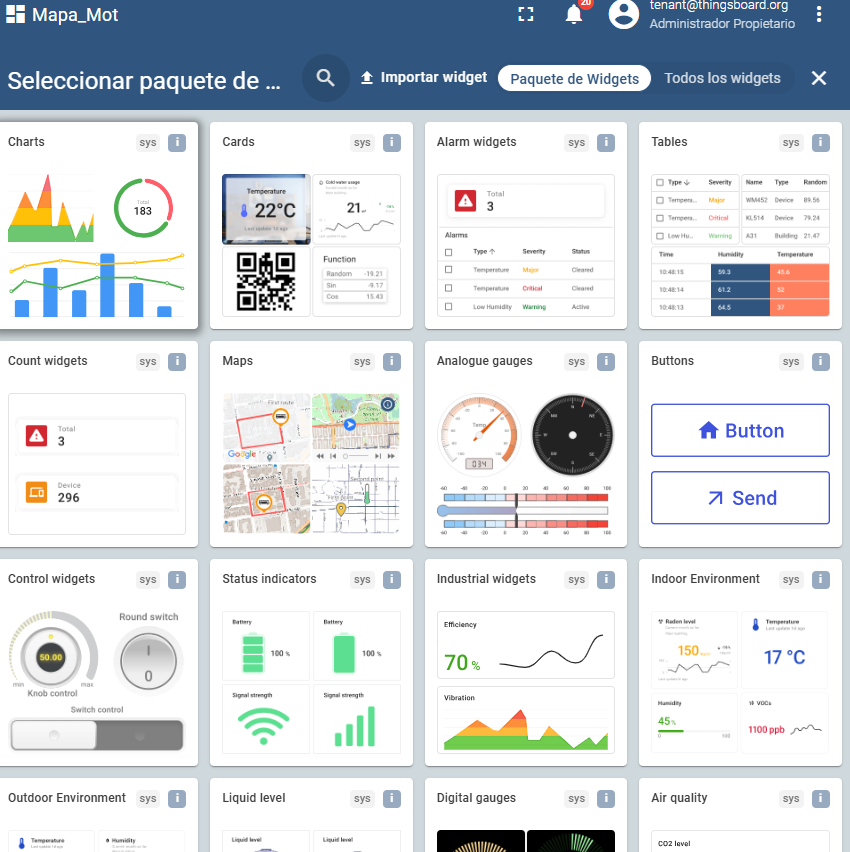
\includegraphics[scale=0.5]{./capitulo_04/imagen/tb/eleccionpanel.png}
\caption{\textit{Widgets} disponibles en \textit{ThingsBoard}. \label{fig:tbpanelelec}}
\end{center}
\end{minipage}
\end{figure}

Se añadieron \textit{widgets} de mapa, como \textit{Route Map - OpenStreet} y \textit{Route Map - Google}, que ofrecen una visualización interactiva de la ubicación en tiempo real (ver Figura \ref{fig:tbdahsboards}). Además, se incorporó un \textit{widget} de tabla de series temporales para analizar datos históricos como latitud y longitud.

\begin{figure}[H]
\leavevmode
\begin{minipage}{\textwidth}
\begin{center}
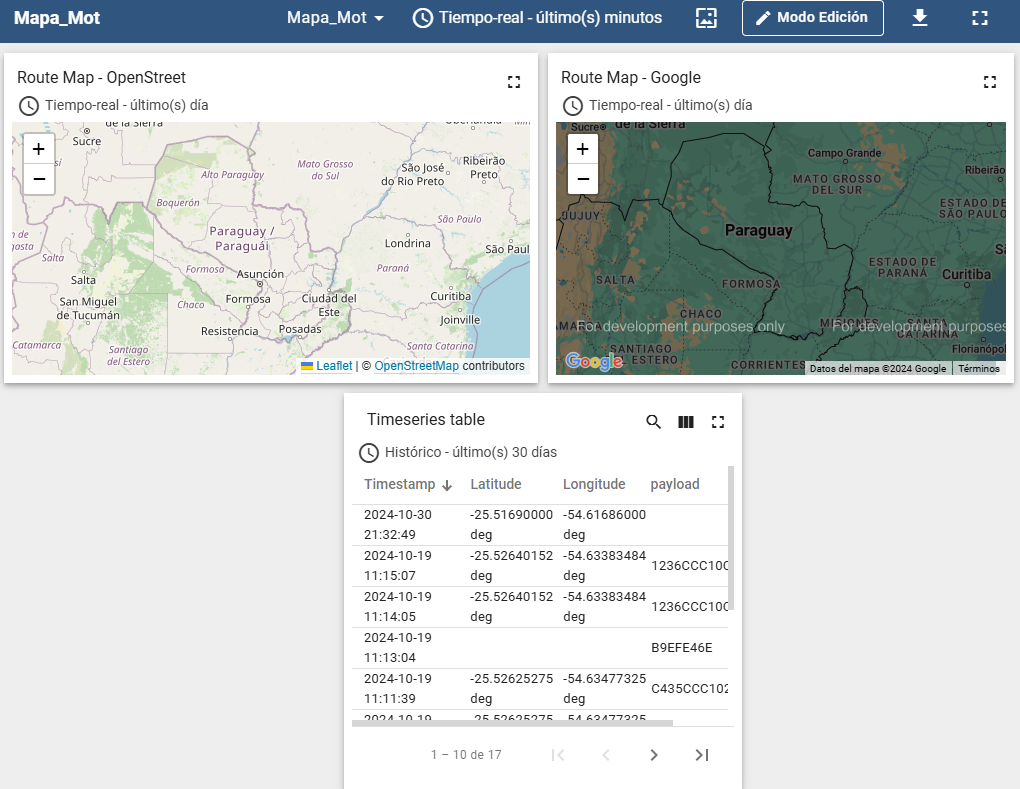
\includegraphics[width=\textwidth]{./capitulo_04/imagen/tb/dahboard.png}
\caption{\textit{Widgets} utilizados en \textit{ThingsBoard}. \label{fig:tbdahsboards}}
\end{center}
\end{minipage}
\end{figure}

Para garantizar la precisión, se configuró una ventana de tiempo en los \textit{widgets}, visualizando información del último día. Se definieron claves como latitud, longitud y estado de actividad para asegurar que los datos mostrados sean precisos (ver Figura \ref{fig:tbpanelconf}).

\begin{figure}[H]
\leavevmode
\begin{minipage}{\textwidth}
\begin{center}
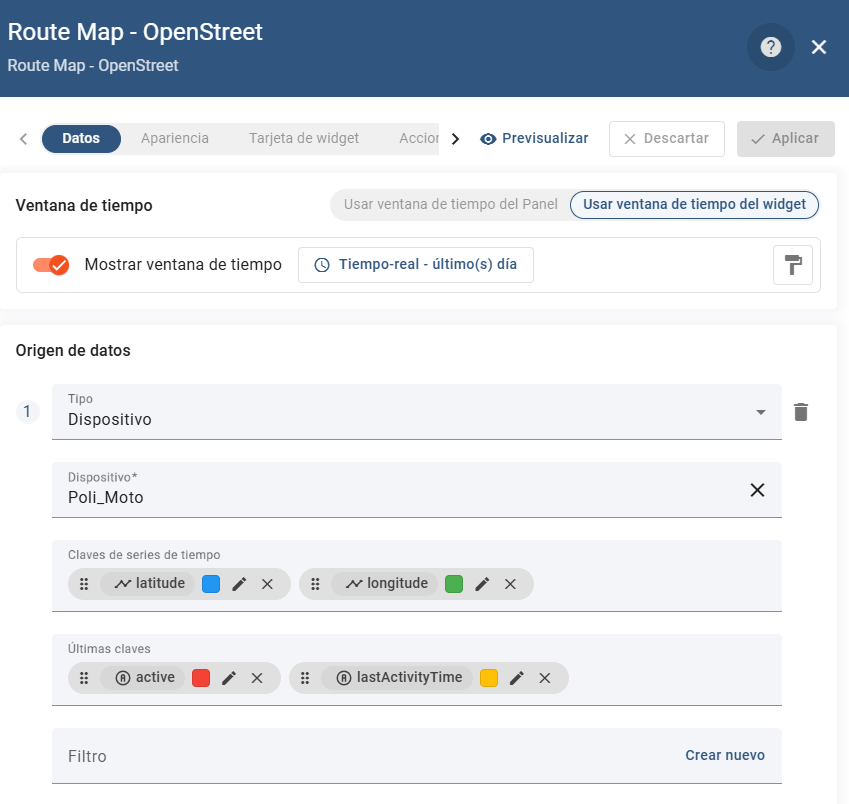
\includegraphics[scale=0.5]{./capitulo_04/imagen/tb/configuracion depanel.png}
\caption{Configuraciones en \textit{Widgets} de Mapa. \label{fig:tbpanelconf}}
\end{center}
\end{minipage}
\end{figure}

\paragraph{Definición de las \textit{Rule Chains} en el Motor de Reglas\\}

En el motor de reglas \textit{(Rule Engine)}, se configuraron cadenas de reglas personalizadas para procesar los mensajes recibidos. Se creó una cadena llamada \textit{MQTT}, con nodos como un decodificador base64 y hexadecimal, para transformar los datos antes de almacenarlos en series temporales (ver Figura \ref{fig:tbruls}).

\begin{figure}[H]
\leavevmode
\begin{minipage}{\textwidth}
\begin{center}
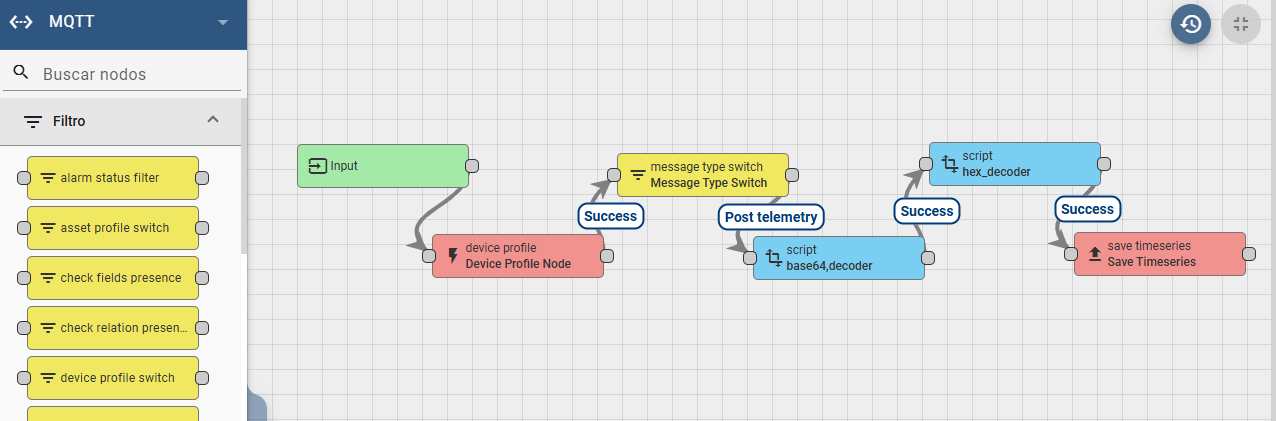
\includegraphics[width=\textwidth, height=0.5\textwidth]{./capitulo_04/imagen/tb/ruleengin.png}
\caption{Diagrama del motor de reglas \textit{MQTT} en \textit{ThingsBoard}. \label{fig:tbruls}}
\end{center}
\end{minipage}
\end{figure}

\paragraph{Configuración de Alarmas y Notificaciones\\}

Se configuraron alarmas para generar alertas en eventos específicos, como desconexiones del dispositivo o valores de telemetría fuera de parámetros. Estas alarmas mejoran la capacidad de respuesta del sistema ante eventos críticos. 

Todas las configuraciones siguieron las mejores prácticas de la documentación oficial de \textit{ThingsBoard} \cite{ThingsBoard_docs2}.




\subsection{Integración de \textit{ThingsBoard} con \textit{Helium}}

La siguiente etapa consistió en la integración de \textit{ThingsBoard} con la consola \textit{Helium}.Para integrar estas herramientas y lograr una transmisión de datos en tiempo real, se configuró una integración a través del protocolo \textit{MQTT}. Este proceso permitió recibir datos de telemetría desde dispositivos conectados a la red \textit{Helium} y visualizarlos en el tablero de \textit{ThingsBoard}. A continuación, se detallan los pasos realizados para establecer esta integración.

Primero, se accedió al menú de \textit{Integrations} en la consola de \textit{Helium}, señalado con la flecha (A) en la Figura ~\ref{fig:integra_hel}. En este menú, se seleccionó la opción para añadir una nueva integración, lo que despliega un conjunto de opciones básicas de integración. Entre estas opciones, se encuentra \textit{MQTT}, identificado con el círculo (B) en la Figura ~\ref{fig:integra_hel}, que fue el protocolo elegido para transmitir los datos de los dispositivos a \textit{ThingsBoard}.

\begin{figure}[H]
\leavevmode
\begin{minipage}{\textwidth}
\begin{center}
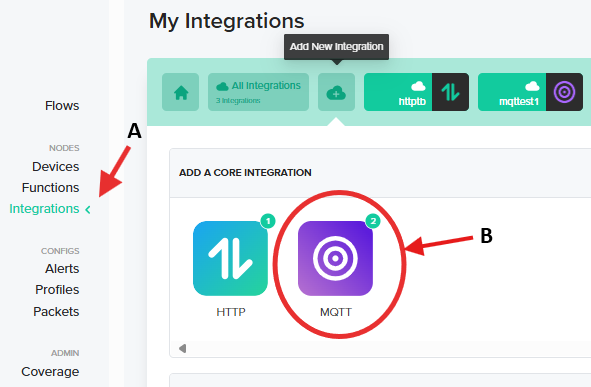
\includegraphics[width=0.7\textwidth]{./capitulo_04/imagen/tb2/hel_integr.png}
\caption{Menú de integraciones en la consola de \textit{Helium}. \label{fig:integra_hel}}
\end{center}
\end{minipage}
\end{figure}


%%comenta

Una vez seleccionada la opción \textit{MQTT}, se procedió a configurar los detalles de conexión en la consola de \textit{Helium}, como se muestra en la Figura ~\ref{fig:mqt_helsl}. En la sección \textit{MQTT} Connection Details, se definieron varios parámetros clave para establecer la comunicación con el servidor de \textit{ThingsBoard}:

En el campo Endpoint, señalado con la etiqueta (A) en la Figura ~\ref{fig:mqt_helsl}, se incluyó el token único del dispositivo generado previamente en \textit{ThingsBoard}, el cual se añadió directamente en la URL como credencial de acceso.
La dirección IP pública del servidor y el puerto estándar para \textit{MQTT} (1883), marcados con la etiqueta (B) en la Figura ~\ref{fig:mqt_helsl}, fueron configurados para garantizar la correcta vinculación con el servicio remoto.
Finalmente, se establecieron los temas necesarios para la comunicación señalados con la flecha (C) en la Figura ~\ref{fig:mqt_helsl}. El tema \textit{Uplink Topic}, fue configurado como v1/devices/me/telemetry, permitiendo el envío de datos de telemetría desde los dispositivos, el tema \textit{Downlink Topic}, se configuró para recibir comandos y configuraciones desde \textit{ThingsBoard} hacia los dispositivos.
Con esta configuración, se garantizó una comunicación bidireccional entre ambos sistemas, facilitando tanto la gestión remota como el monitoreo en tiempo real de los dispositivos conectados.


\begin{figure}[H]
\leavevmode
\begin{minipage}{\textwidth}
\begin{center}
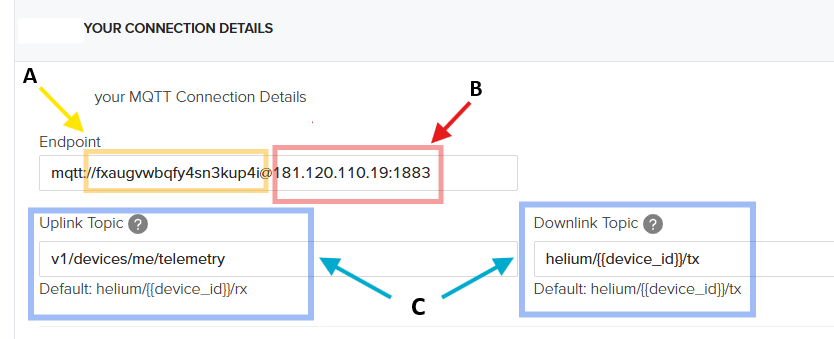
\includegraphics[width=1.0\textwidth]{./capitulo_04/imagen/tb2/detalisconect.png}
\caption{Detalles de conexión \textit{MQTT} configurados en la consola de \textit{Helium}. \label{fig:mqt_helsl}}
\end{center}
\end{minipage}
\end{figure}


Después de configurar los detalles de conexión, se procedió a crear un flujo en la consola de \textit{Helium} que conecta los dispositivos a la integración \textit{MQTT\_TB}, como se observa en la Figura ~\ref{fig:flow}. En el menú Flows (A), se seleccionó la integración previamente configurada, etiquetada como \textit{MQTT\_TB} (B) en la Figura ~\ref{fig:flow}, y se vinculó con el dispositivo PruebaHeltec. Este flujo garantiza que los datos capturados por el dispositivo se envíen automáticamente a \textit{ThingsBoard} a través de la red \textit{Helium}.







\begin{figure}[H]
\leavevmode
\begin{minipage}{\textwidth}
\begin{center}
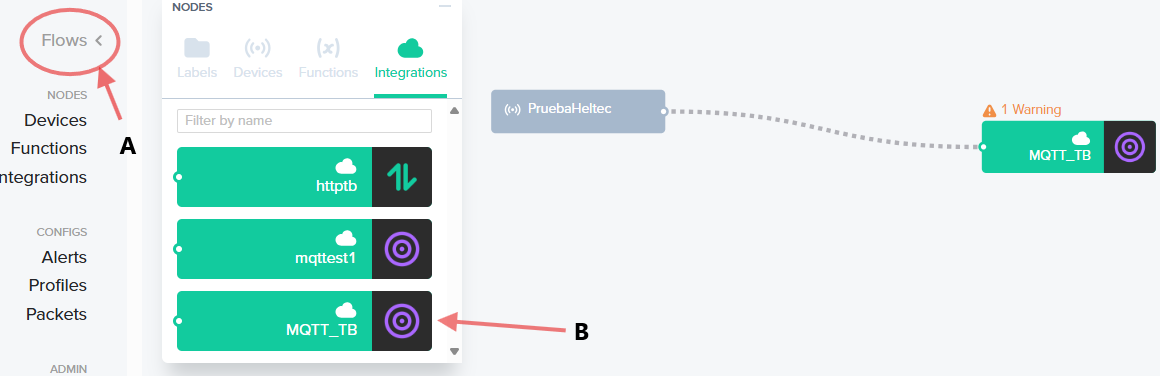
\includegraphics[width=1.0\textwidth]{./capitulo_04/imagen/tb2/flowconf.png}
\caption{Flujo de integración entre el dispositivo PruebaHeltec y \textit{MQTT\_TB}. \label{fig:flow}}
\end{center}
\end{minipage}
\end{figure}

Para completar la integración, fue necesario configurar la redirección de puertos en el router de la red local donde se encuentra alojado el servidor \textbf{ThingsBoard}. En la sección \textit{IPv4 Port Mapping} del panel de administración del \textit{router} (ver Figura~\ref{fig:routconf}, se realizó el mapeo correspondiente para permitir el acceso externo al servidor \textit{MQTT}. Se definió un nombre de mapeo denominado \textit{TBMQTT}, señalado en (A) de la Figura~\ref{fig:routconf}, que asocia la dirección IP interna del servidor (192.168.100.5) con la IP pública asignada a la red (181.94.228.197) indicado con (B) de la Figura~\ref{fig:routconf}). Asimismo, identificado con el círculo (C) en la Figura~\ref{fig:routconf} ,se estableció el puerto 1883 como punto de entrada para las conexiones externas, y se configuró el protocolo TCP, necesario para garantizar la correcta transmisión de los datos.



\begin{figure}[H]
\leavevmode
\begin{minipage}{\textwidth}
\begin{center}
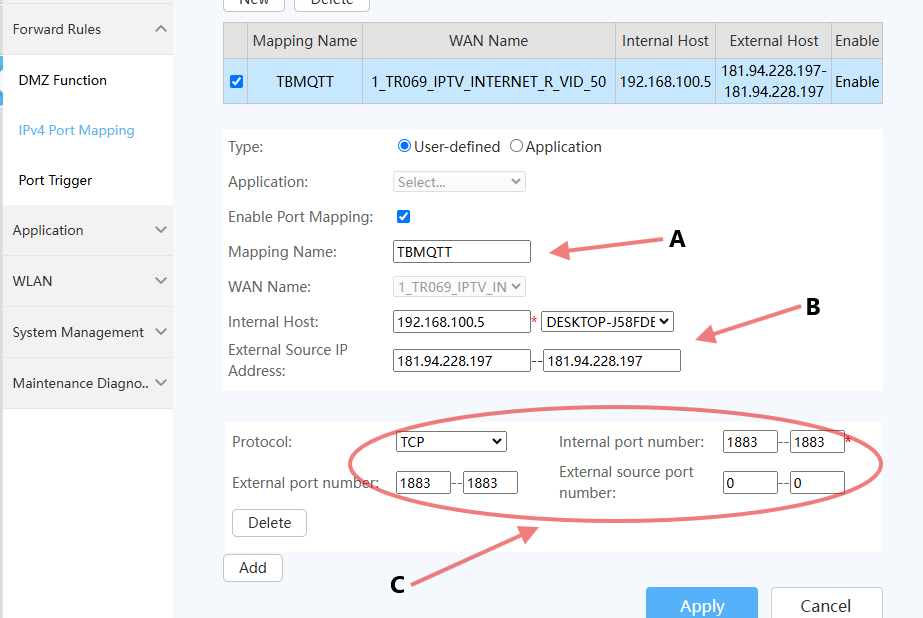
\includegraphics[width=1.0\textwidth]{./capitulo_04/imagen/tb2/rout_conf.png}
\caption{Configuraciones en el \textit{router} de la red local. \label{fig:routconf}}
\end{center}
\end{minipage}
\end{figure}

Con estos ajustes, se completó la integración de \textit{ThingsBoard} con \textit{Helium}, permitiendo que los datos capturados por los dispositivos en la red \textit{Helium} sepuedan transmitir de manera funcional al servidor \textit{ThingsBoard} para su visualización y monitoreo en tiempo real.

\section {Integración de componentes y encapsulamiento}

En esta sección, se describe el proceso de integración de los distintos módulos desarrollados en el sistema y el encapsulamiento final del dispositivo. El objetivo de esta fase es lograr que los módulos de autenticación, control, captura y transmisión de datos trabajen de forma conjunta. Además, se diseñaron un encapsulado protector y estético para asegurar la robustez y usabilidad del dispositivo en su entorno final. A continuación, se detallan las etapas de integración y encapsulado del sistema.

Este proceso se dividio en cuatro etapas:

\begin{itemize}
\item { Implementación Básica con la Integración Inicial entre los Módulos \acrshort{rfid-acronym} y \acrshort{loraw}.}
\item { Implementación alternativa con la Integración ajustada entre los Módulos.} 
\item { Incorporación de Corte de Energía y Simulación de Arranque}
\item { Modelado y Diseño de Encapsulado 3D.}
\end{itemize}


\subsection{Implementación Básica con Integración Inicial de los Módulos \acrshort{rfid-acronym} y \acrshort{loraw}}
En esta primera etapa, se integraron los módulos de autenticación \acrshort{rfid-acronym} y el sistema de comunicación \acrshort{loraw}. El objetivo de esta fase fue asegurar que el sistema pudiera autenticar correctamente los UIDs autorizados y transmitirlos de manera confiable a través de la red \acrshort{loraw}.

Para establecer la comunicación entre el módulo \acrshort{rfid-acronym} y la placa de desarrollo WiFi LoRa 32 V3, se emplearon las mismas conexiones definidas previamente en el módulo de autenticación y control, lo cual permitió mantener una estructura coherente en el diseño. Esta configuración inicial proporcionó las bases para evaluar el correcto funcionamiento de los módulos integrados y realizar los ajustes necesarios en las etapas siguientes.


\subsection{Implementación alternativa con la Integración ajustada entre los Módulos.}

Tras implementar la primera versión del código, se identificaron conflictos en la comunicación SPI entre los módulos \acrshort{rfid-acronym} y \acrshort{loraw}. Se observó que el módulo \acrshort{loraw} utilizaba el protocolo SPI con conexiones definidas internamente en la placa de desarrollo, mientras que el módulo \acrshort{rfid-acronym}, al conectarse externamente mediante SPI, generaba un solapamiento que impedía el funcionamiento coordinado de ambos sistemas.

Para abordar los problemas detectados, se diseñó una nueva versión del código que incorporó una integración alternativa con el uso de un ESP-WROOM-32 dedicado exclusivamente a gestionar el módulo \acrshort{rfid-acronym}. Este ajuste tuvo como propósito lograr que los componentes funcionaran sin interferencias en la comunicación, permitiendo una transmisión estable y una sincronización efectiva entre los módulos.

Para establecer la comunicación entre el módulo \acrshort{rfid-acronym} RC522 y la placa de desarrollo ESP-WROOM-32, se utilizó el protocolo SPI. Las conexiones se realizaron de la siguiente manera: el pin 4 se utilizó como CS (Chip Select), el pin 23(MOSI), el pin 18(SCK), el pin 19(MISO) y el pin 15(RESET). La alimentación se proporcionó a través de los pines VCC y GND.

Para la comunicación entre la placa ESP-WROOM-32 y la Heltec WiFi LoRa 32 V3, se empleó el protocolo UART, con las siguientes conexiones: el pin 48 de la WiFi LoRa 32 V3 se conectó al RX del ESP-WROOM-32, el pin 47 de la WiFi LoRa 32 V3 al TX del ESP-WROOM-32, y los pines GND de ambas placas se unieron para asegurar una referencia común de tierra.

El módulo \acrshort{gnss-acronym} se conectó utilizando las mismas conexiones definidas previamente en el módulo de captura y transmisión de datos. En la figura \ref{fig:diagramadeconexion}, se presenta el diagrama de conexiones empleado para esta configuración.

\begin{figure}[H]
\leavevmode
\begin{minipage}{\textwidth}
\begin{center}
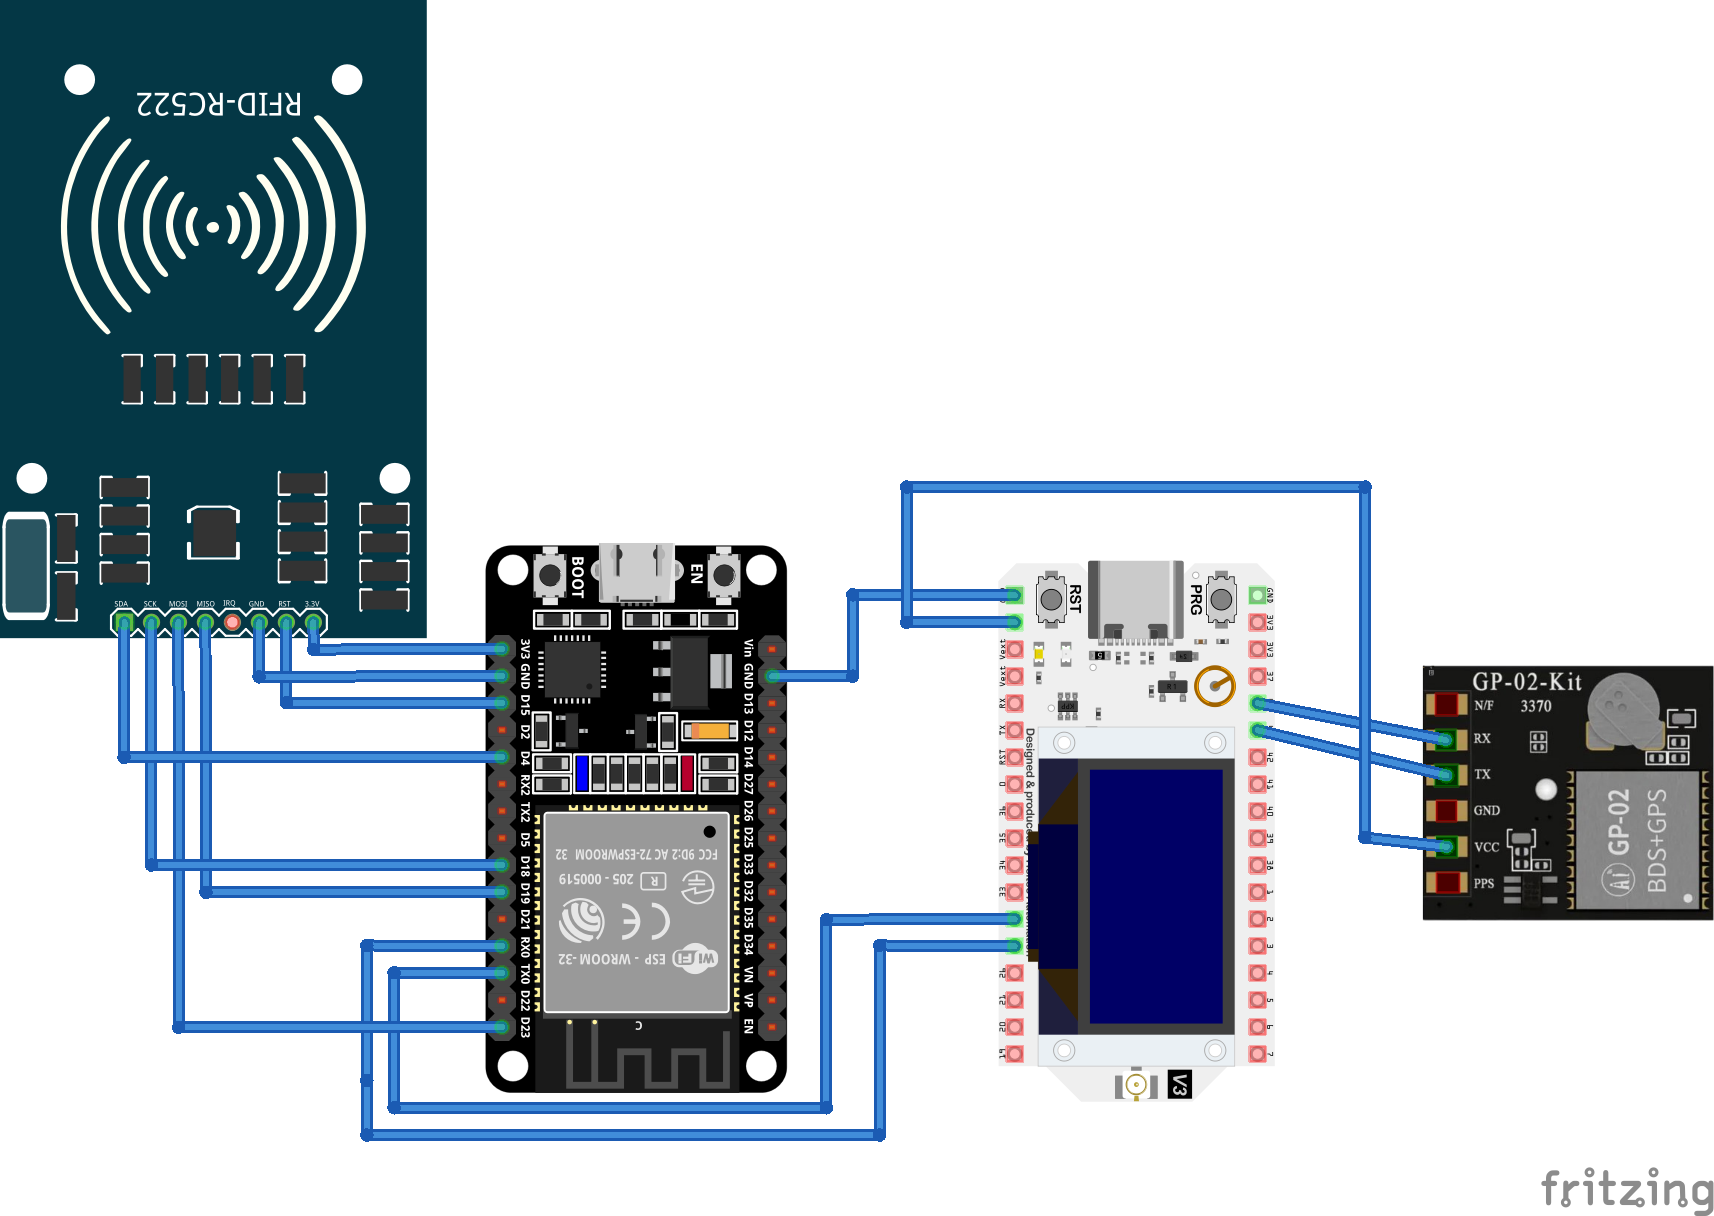
\includegraphics[width=0.7\textwidth]{./capitulo_04/imagen/integracioncompleta.png}
\caption{Diagrama de conexiones entre \acrshort{rfid-acronym} RC522, ESP-WROOM-32, WiFi LoRa 32 V3 y \acrshort{gnss-acronym}.\label{fig:diagramadeconexion}}
\end{center}
\end{minipage}
\end{figure}

Luego de realizar las conexiones, se procedió a ajustar los códigos. En la placa de desarrollo ESP-WROOM-32, se cargó una segunda versión del código previamente desarrollado para el módulo de autenticación y control. Se realizaron modificaciones en el archivo rfidfunciones.cpp, específicamente en la función mostrarUID, que fue adaptada para crear una cadena llamada uidString, la cual almacena el UID en un formato legible.

Durante el procesamiento de cada byte del UID, la función verifica si el valor es menor a 0x10, en ese caso, agrega un 0 al inicio para mantener un formato uniforme. Cada byte se convierte luego a su representación hexadecimal y se añade a uidString, utilizando : como separador entre los bytes. Además, la función almacena cada byte en un array llamado LecturaUID, permitiendo que el UID esté disponible para otras partes del programa cuando sea necesario.

Finalmente, la función imprime el uidString completo en el monitor serial, mostrando el UID del tag \acrshort{rfid-acronym} en el formato deseado para su fácil identificación y verificación.

En esta fase, se añadieron múltiples tareas al sistema para gestionar de manera coordinada la comunicación entre módulos. Estas tareas, cargadas en la placa de desarrollo Heltec WiFi LoRa 32 V3, se organizaron de la siguiente manera:

\begin{itemize}
\item \textbf{Tarea UART (Recepción de Datos \acrshort{rfid-acronym})}: Esta tarea permanece en escucha constante de los datos recibidos desde el módulo \acrshort{rfid-acronym} a través de la UART. Al recibir un UID, este se compara con los UID previamente autorizados. En caso de que el tag recibido sea autorizado, la tarea ajusta el estado del sistema, habilitando el envío del UID por \acrshort{loraw} y activando la tarea de transmisión de \acrshort{loraw}.
\item \textbf{Tarea \acrshort{loraw}}: La tarea de \acrshort{loraw} sigue una máquina de estados que controla las diferentes etapas de transmisión, incluyendo la inicialización, la unión a la red (join), el envío de datos y el ciclo de suspensión (sleep). Esta estructura permite que la tarea transmita los datos de forma programada y que el dispositivo entre en suspensión tras cada transmisión, optimizando así el consumo de energía.
\item \textbf{Tarea GPS}: Esta tarea permanece inactiva hasta que se obtienen coordenadas GPS válidas. Una vez que las coordenadas de latitud y longitud han sido obtenidas y verificadas, la tarea las almacena y las marca como listas para ser enviadas en el siguiente ciclo de transmisión de \acrshort{loraw}. Esto asegura que el sistema envíe únicamente datos de localización precisos.
\end{itemize}


Con los módulos \acrshort{rfid-acronym}, \acrshort{gnss-acronym} y \acrshort{loraw} completamente integrados, se realizaron ajustes finales en el código para definir el funcionamiento general del sistema, que quedó organizado de la siguiente manera:


\begin{itemize}
\item \textbf{Detección \acrshort{rfid-acronym}}: El sistema identifica si un tag \acrshort{rfid-acronym} autorizado está presente. Al detectar un UID autorizado, el sistema se encarga de enviarlo a través de \acrshort{loraw}.
\item \textbf{Envío de Datos por \acrshort{loraw}}: Según el tipo de mensaje seleccionado, puede enviar el UID del \acrshort{rfid-acronym}, otros datos relevantes o, si están disponibles, las coordenadas GPS.
\item \textbf{Ciclo de \acrshort{loraw}}: El sistema opera en un ciclo de transmisión periódico. Durante cada ciclo, envía los datos y luego entra en modo de suspensión (sleep) hasta el siguiente ciclo, optimizando así el consumo energético.
\item \textbf{Validación de Coordenadas GPS}: El sistema realiza intentos continuos de obtener coordenadas GPS válidas. Una vez que estas coordenadas son capturadas con éxito, se preparan para ser enviadas en el próximo ciclo de transmisión de \acrshort{loraw}. 
\end{itemize}


\subsection{ Incorporación de Corte de Energía y de Arranque}

En esta fase, se llevaron a cabo los ajustes finales mediante la incorporación de un módulo de relé, el cual se sincronizó con el módulo \acrshort{rfid-acronym} para gestionar el corte de energía y el arranque del sistema. Para implementar esta funcionalidad, se añadió una nueva tarea al código, denominada vTaskCorriente. Esta tarea permanece a la espera de recibir una notificación que indique el estado del relé. Cuando la notificación recibida desde la tarea UART (Recepción de Datos \acrshort{rfid-acronym}) es positiva, el relé se activa, permitiendo el arranque del sistema, en caso contrario, el relé se desactiva, interrumpiendo la corriente y apagando el sistema. Para ilustrar la estructura y conexiones del sistema, se diseñó un diagrama esquemático completo, que se presenta en la Figura \ref{fig:diagramacompleto}.

\begin{figure}[H]
\leavevmode
\begin{minipage}{\textwidth}
\begin{center}
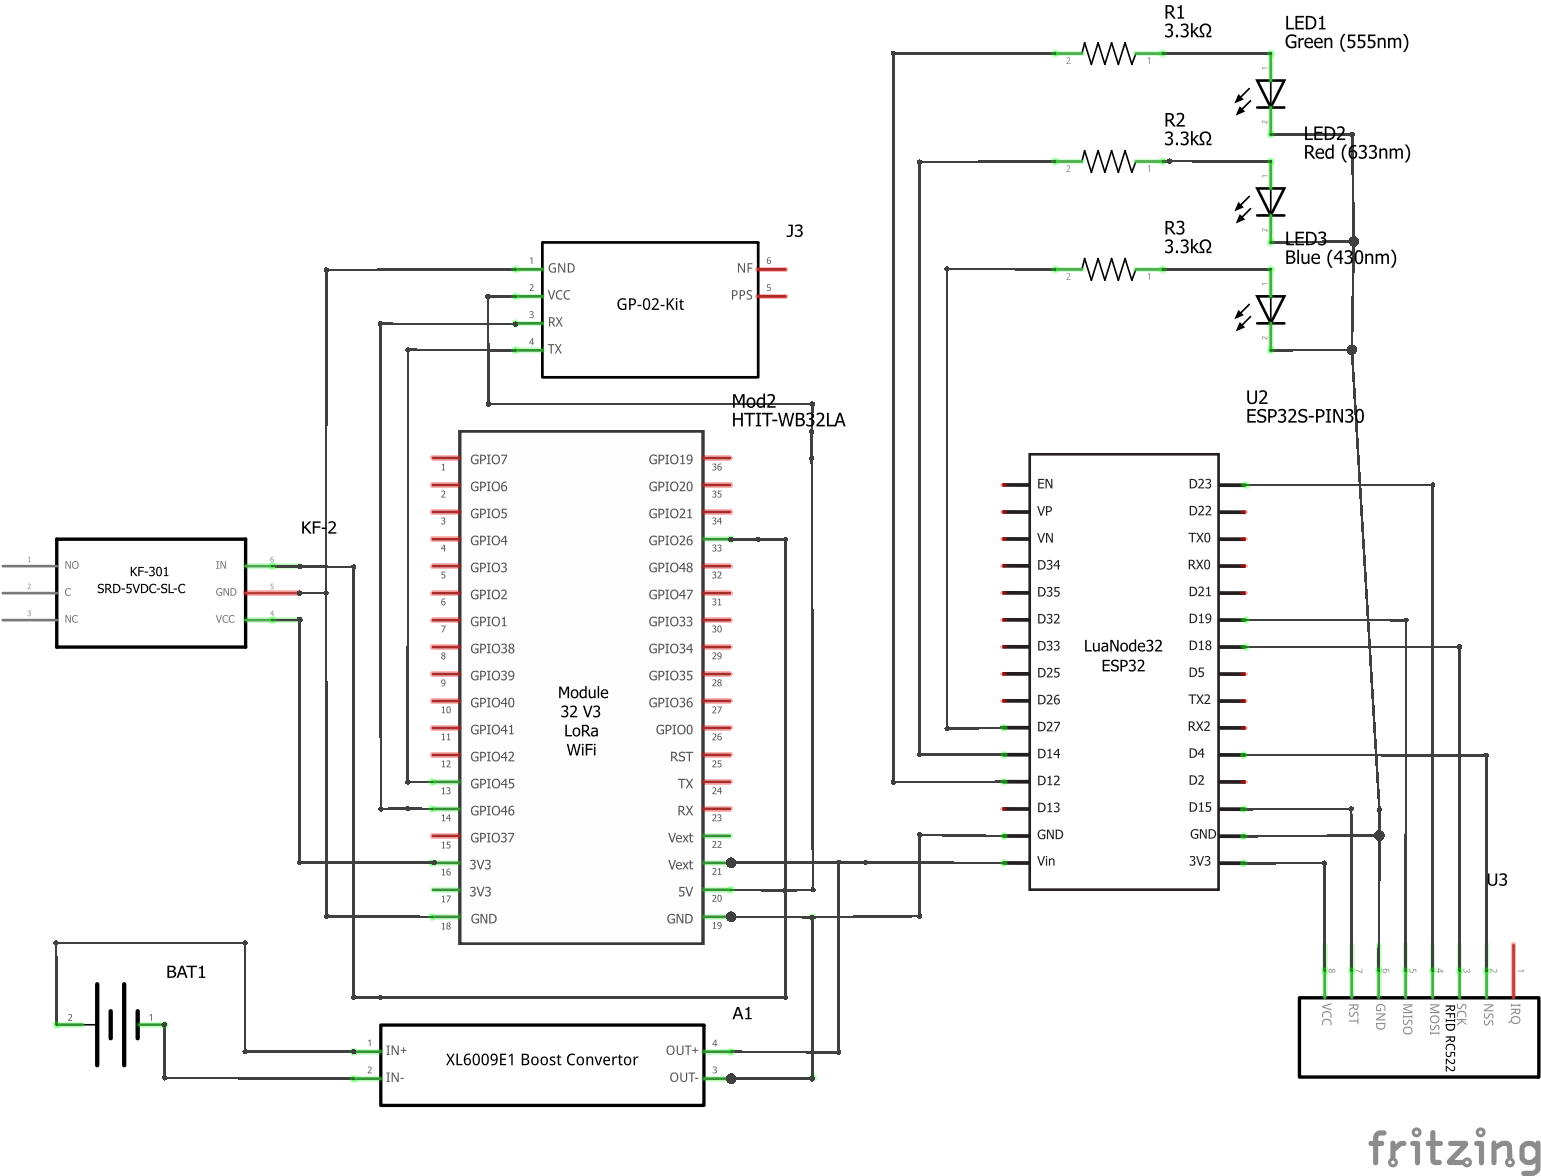
\includegraphics[width=\textwidth]{./capitulo_04/imagen/diagramacompleto.png}
\caption{Diagrama de conexiones de todos los módulos.\label{fig:diagramacompleto}}
\end{center}
\end{minipage}
\end{figure}

Además, se integraron tres LEDs para indicar los estados del sistema. El LED rojo realiza un “self-check” del módulo \acrshort{rfid-acronym}, indicando que este aún no está listo. Una vez completada la inicialización del \acrshort{rfid-acronym}, el LED verde se enciende, señalizando que el sistema está preparado para la lectura. Cuando un tag es detectado y autorizado, el LED azul se enciende para confirmar el acceso. Esta señalización mediante LEDs facilita el monitoreo visual del estado y funcionamiento del sistema en tiempo real.

Por último, se añadió un nuevo tipo de mensaje al sistema de transmisión por \acrshort{loraw} para alertar en caso de desconexión, informando sobre el estado de corte de energía.




\subsection{ Modelado y Diseño de Encapsulado 3D.}

En esta fase, se comenzó definiendo la disposición y estructura de los componentes en el sistema. En primer lugar, se determinó la ubicación óptima de cada módulo, de manera que los elementos clave estuvieran organizados de forma compacta y funcional. Este paso fue esencial para facilitar el acceso a los conectores y puertos de cada componente, optimizando el espacio y garantizando una configuración estructurada.

En la Figura \ref{fig:diseño}, se presenta la distribución de los componentes, donde puede observarse cómo cada módulo está colocado estratégicamente para minimizar el uso de cables y asegurar una accesibilidad adecuada. Esta disposición garantiza que los puertos y conexiones principales sean accesibles para su mantenimiento.


\begin{figure}[H]
\leavevmode
\begin{minipage}{\textwidth}
\begin{center}
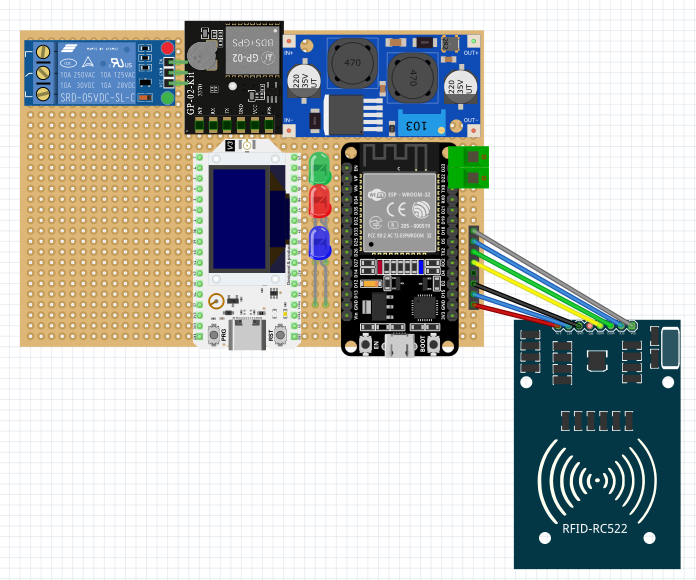
\includegraphics[width=0.6\textwidth]{./capitulo_04/imagen/disposicion.png}
\caption{Disposición estructural de los componentes.\label{fig:diseño}}
\end{center}
\end{minipage}
\end{figure}


Con la disposición estructural establecida, se avanzó a la etapa de diseño del encapsulado 3D mediante el software Blender. Este encapsulado fue modelado específicamente para proteger los componentes, adaptándose a sus dimensiones y ubicación en el shield. La estructura fue diseñada para proporcionar una cobertura robusta y duradera, evitando el movimiento de los componentes internos y protegiéndolos de factores externos.


En la figura \ref{fig:case}, se puede observar el modelo 3D del encapsulado final, que incluye aperturas específicas para cada puerto y conector, así como detalles adicionales para facilitar el montaje y desmontaje de componentes en caso de futuras modificaciones o mantenimientos. 

\begin{figure}[H]
\leavevmode
\begin{minipage}{\textwidth}
\begin{center}
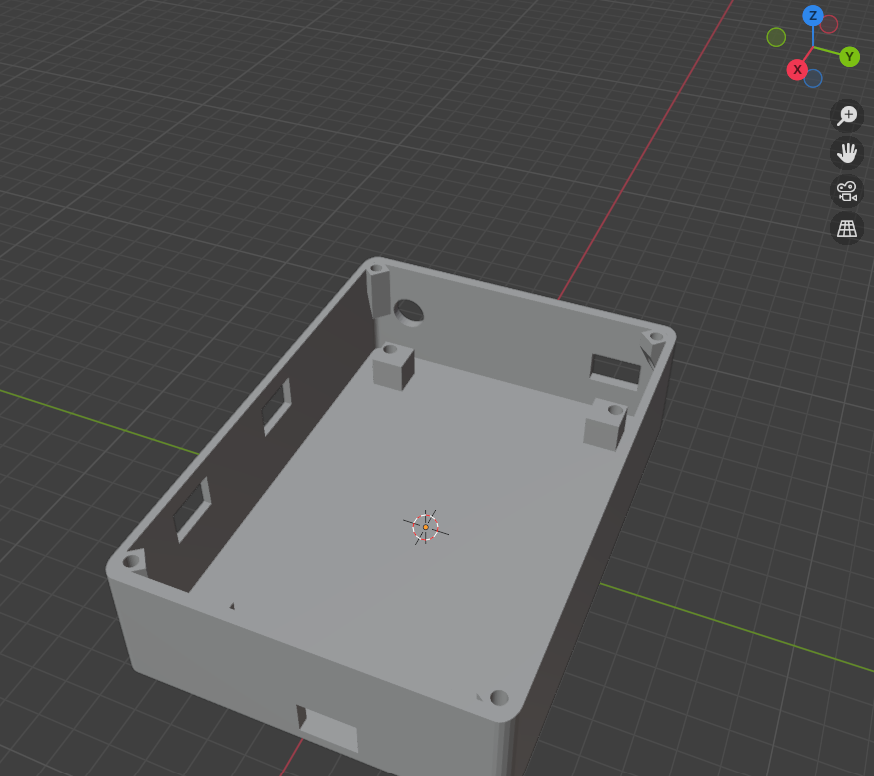
\includegraphics[width=0.6\textwidth]{./capitulo_04/imagen/casebase.png}
\caption{Base del encapsulado.\label{fig:case}}
\end{center}
\end{minipage}
\end{figure}

En la figura \ref{fig:tapa}, se observa el diseño de una tapa destinada a cubrir el encapsulado, proporcionando una capa adicional de protección para los componentes internos. Esta tapa fue modelada para ajustarse de forma precisa al contorno del encapsulado, incluyendo accesos a los conectores que permiten la salida de los cables necesarios para el funcionamiento del sistema.


\begin{figure}[H]
\leavevmode
\begin{minipage}{\textwidth}
\begin{center}
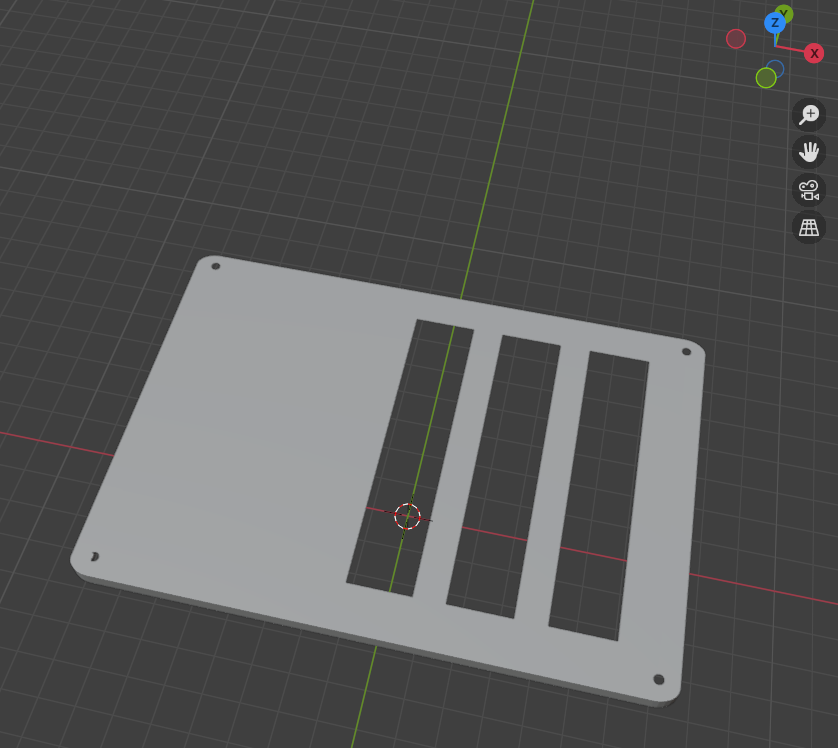
\includegraphics[width=0.6\textwidth]{./capitulo_04/imagen/tapa.png}
\caption{Parte superior del encapsulado.\label{fig:tapa}}
\end{center}
\end{minipage}
\end{figure}


Adicionalmente, se desarrolló un diseño 3D complementario para el módulo \acrshort{rfid-acronym} con el propósito de satisfacer la necesidad de identificación del usuario y garantizar una lectura continua del tag. En la Figura \ref{fig:orificio}, se muestra el diseño del encapsulado, el cual incorpora un orificio estratégicamente ubicado para alojar el tag en una posición fija. Este diseño asegura su permanencia dentro del rango de lectura, optimizando la funcionalidad del sistema y mejorando su integración con los demás componentes.

\begin{figure}[H]
\leavevmode
\begin{minipage}{\textwidth}
\begin{center}
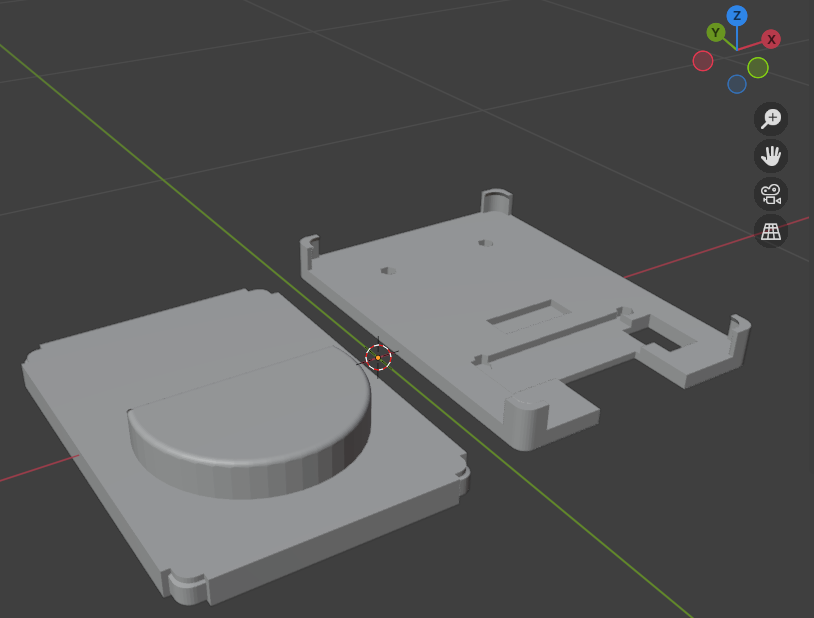
\includegraphics[width=0.6\textwidth]{./capitulo_04/imagen/rfidcaseblender.png}
\caption{Modelado 3D del encapsulado para el módulo \acrshort{rfid-acronym}.\label{fig:orificio}}
\end{center}
\end{minipage}
\end{figure}